Betrachten Sie folgendes Aktivitätsdiagramm:



\begin{centering}
\includegraphics[min width=0.4\textwidth=0.6\textwidth,min height=0.4\textwidth=0.6\textwidth,keepaspectratio,max width=0.9\textwidth,max height=0.9\textwidth]{71/Diagram.pdf}\end{centering}

Betrachten Sie folgendes Petrinetz als Übersetzung dieses Aktivitätsdiagramms:



\begin{centering}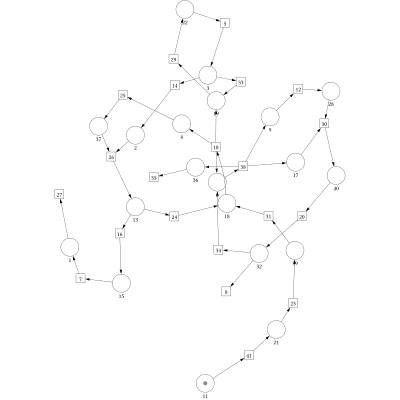
\includegraphics[min width=0.4\textwidth=0.6\textwidth,min height=0.4\textwidth=0.6\textwidth,keepaspectratio,max width=0.9\textwidth,max height=0.9\textwidth]{71/petri0a27d7cfdbb293c5610aa80b6871b353cfc5757a784efcf3be7a07f6a303ff9811014.pdf}\end{centering}

Geben Sie alle Aktionsknoten/Petrinetzknoten-Paare, alle Objektknoten/Petrinetzknoten-Paare, die Petrinetzknoten je anderer Elementart und alle Hilfsstellen und -transitionen im Petrinetz an.

Geben Sie dazu Ihre Antwort wie im folgenden Beispiel an:\begin{verbatim}MatchPetriSolution {actionNodes = [("A",1),("B",2)], objectNodes = [("C",3),("D",4)], decisionNodes = [5,7], mergeNodes = [6,8], forks = [10], joins = [11], initialNodes = [12], activityFinalNodes = [16], flowFinalNodes = [], auxiliaryPetriNodes = [13,14,15]}\end{verbatim}In diesem Beispiel sind etwa die Aktionsknoten "A" und "B" den Petrinetzknoten 1 und 2 zugeordnet, die Petrinetzknoten 5 und 7 entsprechen Verzweigungsknoten, die Petrinetzknoten 13, 14 und 15 sind Hilfsstellen oder -transitionen, der Petrinetzknoten 16 entspricht einem Aktivitätsende und kein Petrinetzknoten entspricht einem Flussende.

Hinweis zur Übersetzung in ein Petrinetz: Für Endknoten werden keine zusätzlichen Stellen eingeführt. Sie werden so realisiert, dass ein Token verbraucht wird, also an dieser Position aus dem Netz verschwindet. Falls eine zusätzliche Transition erforderlich ist, um dieses Verhalten an einer Position im Diagramm zu realisieren, an der sich ein Endknoten befindet, zählt diese Transition nicht als Hilfsknoten.

